\documentclass[11pt]{article}

\usepackage[margin=1in,footskip=0.25in]{geometry}

%\usepackage{helvet}
%\renewcommand{\familydefault}{\sfdefault}

\renewcommand\refname{\vskip -1cm}

%\renewcommand{\rmdefault}{phv} % Arial
%\renewcommand{\sfdefault}{phv} % Arial
\usepackage{setspace}
\usepackage{wrapfig}
\usepackage{amsmath}
\usepackage{amssymb}
\usepackage{graphicx}
\usepackage{mathrsfs}
\usepackage{bm}
\usepackage{wasysym}
\usepackage{placeins}
\usepackage{multirow}
\usepackage[T1]{fontenc}
\usepackage[super]{natbib}
\usepackage{framed}
\usepackage{caption}
\usepackage{longtable}

\begin{document}

\title{Tissue isotope dynamics}

\maketitle

\section{Methods}

\subsection{Isotopic dynamics of a resource specialist}

We start by considering a set of prey items, each with its own range $\delta^{13}C$ and $\delta^{15}N$ values, which we (for now) assume are independent and normally distributed.
We then consider a consumer that selects among these prey items and integrates the isotopic values of prey into its tissues.
The integration of the isotopic values of a prey item is thus a weighted average of the consumer's isotopic values and the isotopic values of the prey, with respect to the different mass of each.

For simplicity, we will assume that a single prey item is consumed over the course of a day.
Even though prey individuals are of different sizes, we will assume that the biomass of consumed prey is the same over the course of each day (i.e. that the consumer is replacing the energy that it spends). 
If $X_c$ is the isotopic value of the consumer, and $X_p$ is the isotopic value of a prey, then

\begin{align}
	X_c(t+1) &= \frac{M_c}{M_c + M_p}X_c(t) + \frac{M_p}{M_c + M_p}X_p(t) \\ \nonumber
	&= fX_c(t) + (1-f)X_p(t)
\end{align}

\noindent where $f$ is the proportion of total biomass that is the consumer's body tissues at the end of the day (i.e. minus body mass spent via metabolism).
The change over time is then

\begin{align}
\label{diffeq}
	X_c(t+1) - X_c(t) &= fX_c(t) + (1-f)X_p(t) - X_c(t),~~\mbox{equivalent to} \\
	\frac{\rm d}{\rm dt}X_c &= fX_c + (1-f)X_p - X_c,
\end{align}

\noindent in continuous time. 
The above differential equation describes how the consumer's biomass changes as it incorporates the mass of some prey $p$.
Note that - for now - we are assuming that the consumer is specializing on a single prey.
Solving for Eq. \ref{diffeq} reveals a tissue incorporation decay curve $X_c = X_p + (X_0-X_p)\exp\{(f-1)t\}$, where a tissue starts with an isotope value $X_0$ and at the limit $t\rightarrow \infty $, we find that $X_c \rightarrow X_p$, which means that the consumer's isotope value eventually approaches that of its only prey... it had better!

This is the exciting part! So far, we have assumed that the prey isotope value is constant, though we know that prey isotope values have variability.
We want to incorporate this idea that prey isotope values are variable, and then solve for the mean (expectation) and variability of the consumer as it eats its prey.
Just a reminder: the consumer is still a specialist, consuming a single, but variable prey.

So in this next section, we assume that $X_p \sim {\rm Norm}(\bar{x}_p,\sigma^2)$, meaning the $X_p$ is a random variable normally distributed about a mean value $\bar{x}_p$ with variance $\sigma^2$.
Then, we have to rewrite Eq. \ref{diffeq} as a Stochastic Differential Equation, which is badass

\begin{equation}
	{\rm dX_c} = fX_c{\rm dt} + (1-f)(\bar{x}_p{\rm dt} + \sigma{\rm dW}) - X_c{\rm dt}
\end{equation}

\noindent where everything is as before, except that we have this funky term to the right of $(1-f)$, which basically says that the prey isotope value varies over time (as different individuals of the same prey are consumed), and that this variability scales with $\sigma$, which is the standard deviation of the prey's isotope value, while ${\rm dW}$ is the increment of Brownian motion.

We can then solve for the expectation and variability of the consumer's isotope value (${\rm E}\{X_c\}$ and ${\rm Var}\{X_c\}$, respectively).
We find that

\begin{align}
	{\rm E}\{X_c(t)\} &= \bar{x}_p + (X_0-\bar{x}_p){\rm e}^{-(1-f)t}, \nonumber \\ \nonumber \\ 
	{\rm Var}\{X_c(t)\} &= \frac{\sigma^2(f-1)}{2}({\rm e}^{-2(1-f)t} -1).
\end{align}

\noindent As before, in the limit of $t \rightarrow \infty$, ${\rm E}\{X_c\} \rightarrow \bar{x}_p$, such that the specialist consumer will be centered around its prey.
The most interesting result is that as $t \rightarrow \infty$, ${\rm Var}\{X_c\} \rightarrow \sigma^2(1-f)/2$.
Because $0 < f \leq 1$, this means that the variance of the consumer will always be less than the variance of the prey ($\sigma^2$).
The degree to which the consumer's variance is less than the prey's variance is due primarily to $f$, which describes the proportional difference between the mass of the consumer vs. the ingested resource.

\subsection{Isotopic dynamics of a prey-switching consumer}

Now let's consider the case of a consumer that can incorporate multiple prey into its diet over the course of each day.
The primary change is that -- rather than sampling from a single prey isotopic distribution, and incorporating this sample into the consumer's mass -- we are sampling from multiple prey isotopic distributions.
We also want to retain enough flexibility in the design so that we can simulate on one end a specialist consumer (as before), and on the other end a generalist consumer, as well as everything in between.

To do this, we can assume that within each time step, the consumer incorporates a certain proportion of each prey, so that it is integrating $Z = \sum_{i=1}^Np_iX_i$, where $p_i$ is the proportional contribution of the isotope value $X$ for prey $i$, summed over the $N$ available prey.
As before, we assume that $X_i$ is normally distributed ($X_i \sim {\rm Norm}[\bar{x}_i, \sigma_i^2]$), and that each prey's distribution is independent of the others.
We also want to assume that $p_i$ is a random variable, such that an individuals behavior can change over time.
Because $\sum_{i=1}^N p_i = 1$, these variables are not independent.

The random proportional contribution vector $\bm p$ (of which $p_i$ is a single element, such that the vector sums to one) is distributed as a Dirichlet Distribution, which is an $N$-dimensional distribution where the individual elements can range from 0 to 1.
The Dirichlet distribution is parameterized by the vector $\bm a$, where each element has a value greater than or equal to one.
If all $a_i = 1$, the distribution is flat.
If all $a_i = 1$, except for one element, which has an arbitrarily high number, the proportional contribution of that prey item will be large, whereas the rest will be low.
As such, the mean proportional contribution of each prey item, as given by a particular Dirichlet distribution is

\begin{equation}
	{\rm E}\{p_i\} = \frac{a_i}{a_0}.
\end{equation}

\noindent where $a_0 = \sum_{i=1}^N a_i$.
The variance of the proportional contribution of each prey item is then

\begin{equation}
	{\rm Var}\{p_i\} = \frac{a_i(a_0 - a_i)}{a_0^2(a_0 + 1)}.
\end{equation}

This is where things get tricky.
Because the isotopic value that the consumer is integrating is now $Z = \sum_{i=1}^Np_iX_i$, where both $p_i$ and $X_i$ are random variables, we need to estimate the mean and variance of $Z$ so that we can integrate this into the stochastic differential equation framework.
When we put it all together, the stochastic differential equation is

\begin{equation}
{\rm d}X_c = (f-1)X_c{\rm dt} + (1-f)\left({\rm E}\{Z\} {\rm dt} + \sqrt{{\rm Var}\{Z\}}{\rm dW}\right).
\end{equation}

There is some funny business about stochastic differential equations that we don't need to get into: because the timesteps are infinitely small, the variance of Brownian motion is infinitely large.
The important point is that no matter what distribution you are sampling from, because of the central limit theorem, $X_c$ will be normally distributed at the long time limit.
So assuming $Z \sim {\rm Norm}\{{\rm E}\{Z\}, \sqrt{{\rm Var}\{Z\}}\}$ -- even if $Z$ isn't normally distributed by itself -- is correct.
So now we want to find ${\rm E}\{Z\}$ and ${\rm Var}\{Z\}$.
After much pain, we find

\begin{equation}
	{\rm E}\{Z\} = \sum_{i=1}^N \bar{p}_i \bar{x}_i	
\end{equation}

\noindent where $\bar{p}_i$ and $\bar{x}_i$ are the means of each, respectively.
Moreover (and this was the painful part),

\begin{equation}
	{\rm Var}\{Z\} = \sum_{i=1}^N {\rm Var}\{p_i\}{\rm Var}\{X_i\} + \bar{p}_i^2{\rm Var}\{X_i\} \bar{x}_i^2 {\rm Var}\{p_i\} + \sum_{\substack{
	j=1 \\
	j \neq i}							
	}^N {\rm Cov}\{p_ip_j)\bar{x}_i\bar{x}_j,
\end{equation}

\noindent where 

\begin{equation}
	{\rm Cov}\{p_i,p_j\} = \frac{-a_ia_j}{a_0^2(a_0 + 1)}.
\end{equation}

Now we have an explicit formulation for the means and variances of $Z$, and to get back at estimating the expectation and variance for $X_c$ (the goal in all of this), we can plug these values back into the original solution for the specialist case, such that

\begin{align}
	{\rm E}\{X_c(t)\} &= \sum_{i=1}^N \bar{p}_i \bar{x}_i + \left(X_0-\sum_{i=1}^N \bar{p}_i \bar{x}_i\right){\rm e}^{-(1-f)t}, \nonumber \\ \nonumber \\ 
	{\rm Var}\{X_c(t)\} &= \frac{{\rm Var}\{Z\}(f-1)}{2}\left({\rm e}^{-2(1-f)t} -1\right).
\end{align}

\noindent as $t\rightarrow \infty$, we find that 

\begin{align}
	{\rm E}\{X_c(t\rightarrow \infty)\} &= \sum_{i=1}^N \bar{p}_i \bar{x}_i, \nonumber \\ \nonumber \\ 
	{\rm Var}\{X_c(t\rightarrow \infty)\} &= \frac{{\rm Var}\{Z\}(1-f)}{2}.
\end{align}

{\bf Initial insights}

\begin{enumerate}
\item The asymptote in variance occurs quickly (at rate $(1-f)$ for the expectation, and at rate $2(1-f)$ for the variance)
\item The variance of a consumer is a fixed amount less than the variance of its component prey
\item The amount that variance is lowered in the consumer is a function of the incorporation rate $(1-f)$ 
\item All we need to solve all of this is means and stdevs of the prey + the Dirichlet parameter set for the consumer (which describes its prey-preferences)
\end{enumerate}


\subsection{The equations for a population (beta)}
So far, we have just calculated properties for a single consumer, but we really care about a population of consumers.
Such a population can vary in a number of cool ways... it could be composed entirely of generalist consumers, it could have specialist consumers that all eat the same thing, it could have specialist consumers that all eat different things, or anything in between.

Because we have analytical expressions for the individual-level moments of the isotopic distributions, we now want to scale up.
Because each individual consumer has normally distributed isotope values, the population is a mixture distribution of multiple normals.
If there are $M$ consumers in the population, the expectation for the population is simple, and is just

\begin{equation}
{\rm E}\{X_{\rm pop}\} = \frac{1}{M}\sum_{k=1}^M \bar{x}_c^{(k)},
\end{equation}

\noindent where $\bar{x}_c^{(k)}$ is the expectation for the kth consumer.
The variance is a little tricker (as always), and is

\begin{equation}
{\rm Var}\{X_{\rm pop}\} = \frac{1}{M^2}\left(\sum_{k=1}^M M {\rm Var}\{X_c^{(k)}\} + (M-1)	\bar{x}_c^{(k)2} - \sum_{\substack{
	l=1 \\
	l \neq k}							
	}^M  \bar{x}_c^{(l)} \bar{x}_c^{(k)} \right).
\end{equation}

\noindent I haven't yet tested the population-level equations, but I'm fairly sure they are right.


\subsection{Injecting more reality} 

Time: Seth pointed out that it would be nice to have real time units.
I think that this dynamic equation is general enough that time is just a scalar, and we can easily fix $f$ to reflect different consumption rates of prey.
For the simulations represented in the figures, I'm assuming that a sea otter weighs 20 kg at the end of the day, and that 1 kg of prey is consumed per day... so the `steady state' body mass is 21 kg.
These can be easily changed to reflect different scenarios.

Different tissues: In the above examples, we were mainly exploring how variance changed with time, and what the limit of variance would be.
The next step is to think about how different tissues accrue variability over different slices of time.
One interesting observation is that variance asymptotes really quickly.
This might be similar variability in liver vs. bone wouldn't be surprising, but needs to be explored further.
I think the tools above will be a flexible skeleton with which we can investigate the more interesting questions (such as tissues-specific variability), which are the real aim of the project.

Prey-switching: The above dynamics only apply to specialist consumers. I'm toying around with ways of generalizing foraging dynamics... I don't yet have a feel as to whether the above analyses will blow up or not when we include this, but it's in progress!

{\bf Thoughts, comments, suggestions, edits, questions?}


\begin{figure*}[h!]
   \centering
   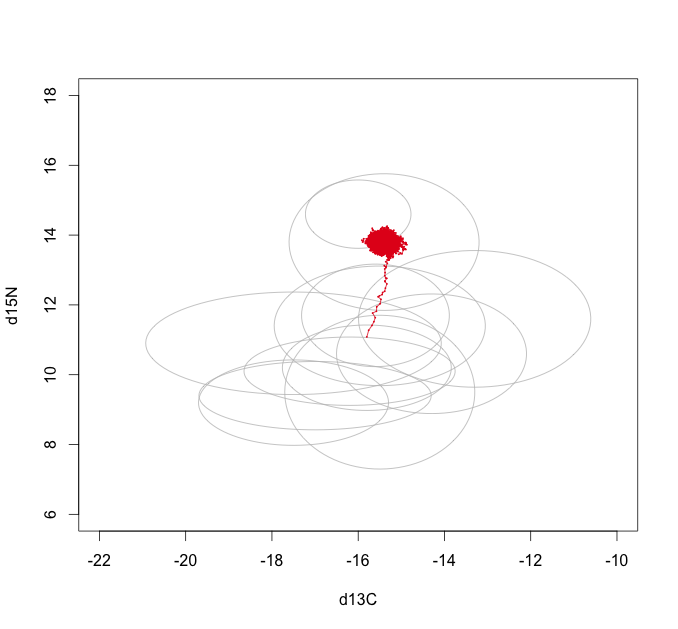
\includegraphics[width=0.5\textwidth]{fig_bivariate.png}
      \caption{
      A consumer (red) incorporating the isotopic values of a single prey species. The starting isotopic values are at the centroid of the prey space. The variability of the consumer is notably smaller than that of its prey.
      }
      \label{fig_bivariate}
\end{figure*}

\begin{figure*}[h!]
   \centering
   \includegraphics[width=0.5\textwidth]{fig_d13CvsTime.png}
      \caption{
      A) The $\delta^{13}{\rm C}$ values of the simulated specialist consumer over time (gray points). The analytical approximation is the black line.
      B) Variability of $\delta^{13}{\rm C}$ values for the simulated forager over time. Bins are set to 200 steps; the smaller the bin, the less accurate the measure of SD.The analytical approximation for variability is the black line.
      }
      \label{fig_time}
\end{figure*}

\begin{figure*}[h!]
   \centering
   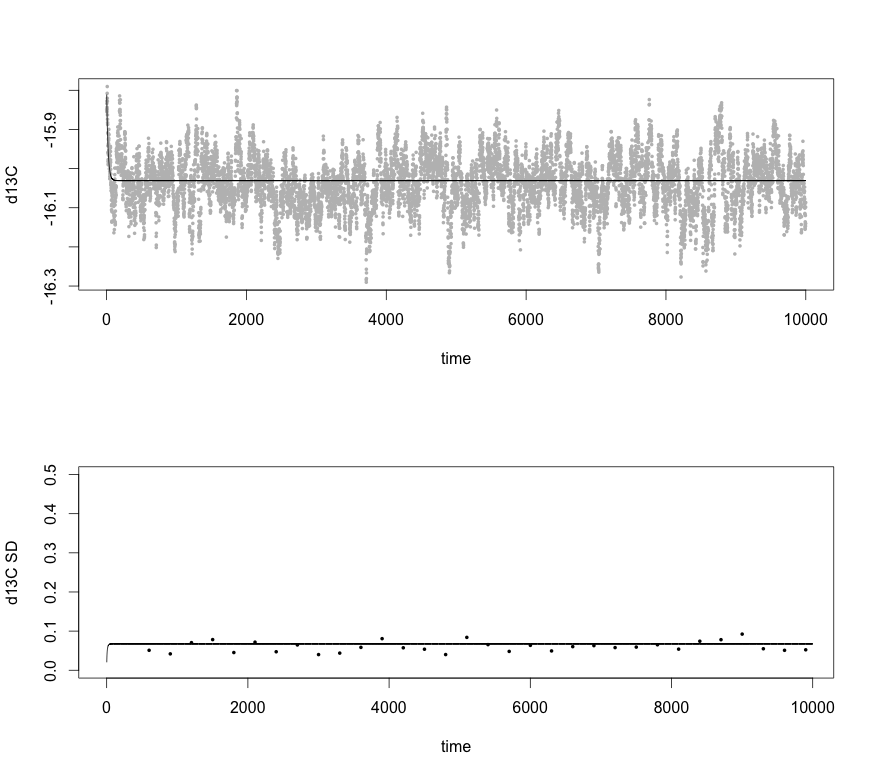
\includegraphics[width=0.5\textwidth]{fig_d13CvsTime_gen.png}
      \caption{
      A) The $\delta^{13}{\rm C}$ values of the simulated consumer with complex prey-switching (it generalizes over most prey, and specializes on three) over time (gray points). The analytical approximation is the black line.
      B) Variability of $\delta^{13}{\rm C}$ values for the simulated forager over time. Bins are set to 300 steps; the smaller the bin, the less accurate the measure of SD. The analytical approximation for variability is the black line.
      }
      \label{fig_time}
\end{figure*}

\begin{figure*}[h!]
   \centering
   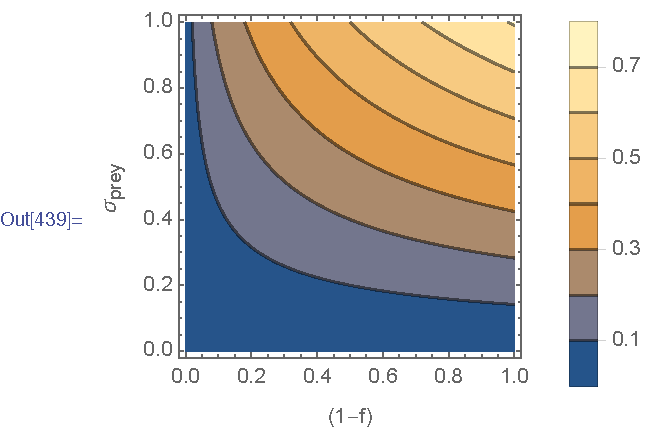
\includegraphics[width=0.5\textwidth]{fig_fvsSigma.pdf}
      \caption{
      The relationship between: x-axis: the incorporation rate $(1-f)$, y-axis: the consumed prey's standard deviation, and z-axis (colors): the standard deviation of the consumer at the asymptotic limit.
      As the incorporation rate increases (such as for fast-turnover tissues), there is greater variance in the consumer for a given variance of consumed prey.
      }
      \label{fig_time}
\end{figure*}




\end{document}
